\documentclass[a4paper,parskip,headheight=38pt]{scrartcl} % article or scrartcl
\usepackage[utf8]{inputenc}
\usepackage{amsmath,amssymb,amsfonts}
\usepackage[%
  automark,
  headsepline                %% Separation line below the header
]{scrlayer-scrpage}
\usepackage[english]{babel}
\usepackage{hyphenat}
\usepackage[hidelinks]{hyperref}
\usepackage[top=1.4in, bottom=1.5in, left=1in, right=1in]{geometry}
\usepackage{lastpage}
\usepackage{csquotes}
\usepackage{microtype}
\usepackage{datetime}

\usepackage[normalem]{ulem}
\usepackage{enumerate}
\usepackage{hyperref}

% \usepackage{multicol}
\usepackage{graphicx}
\usepackage{graphics}
% \usepackage{float}
% \usepackage{caption}

\setkomafont{pagehead}{\normalfont\sffamily\footnotesize}
\addtolength{\headheight}{+6pt}
\lohead{Ben Wiederhake, s9bewied@\ldots, 2541266}
\rohead{ES16, Set 1, Page {\thepage}/{\pageref*{LastPage}}}

\newtimeformat{mytime}{\twodigit{\THEHOUR}\twodigit{\THEMINUTE}\twodigit{\THESECOND}}
\settimeformat{mytime}
\newdateformat{mydate}{\twodigit{\THEYEAR}\twodigit{\THEMONTH}\twodigit{\THEDAY}}
\cfoot{\tiny\texttt{ID \mydate\today\currenttime}}
\chead{} % Needed because now the \subsections get displayed
\pagestyle{scrheadings}

% \renewcommand{\headrulewidth}{0pt}
% \addtolength{\textheight}{+30mm}
% \addtolength{\textwidth}{+50mm}
% \addtolength{\hoffset}{-7mm}

% \newcommand{\Omicron}{\ensuremath{\mathcal{O}}}
% \newcommand{\omicron}{\ensuremath{o}}
% \newcommand{\set}[1]{\{#1\}}
% \newcommand{\abs}[1]{\lvert #1 \rvert}

\begin{document}

\section*{Problem 1: Simulink}

\subsection*{Part 1: Sketch}

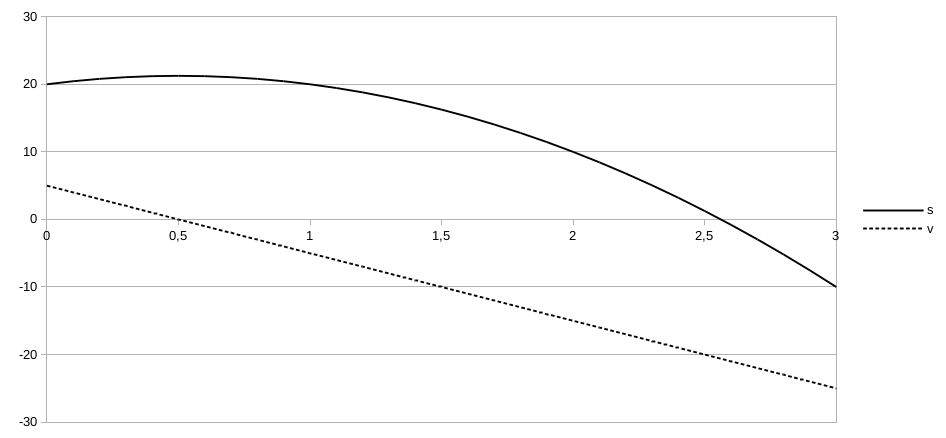
\includegraphics[width=\textwidth]{p1-sketch}

\subsection*{Part 2: Differential equations}

\begin{align*}
    v(0) &= 5 \\
    dv/dt &= -10 \\
    s(0) &= 20 \\
    ds/dt &= v(t)
\end{align*}


\section*{Problem 2: Car Motion on a Slope}

In order to be an equilibrium, the state must have $\dot{x} = 0 \land
\dot{v} = 0$, which implies $v=0$ and (with $v=0$ already applied) $-g
\sin \theta = 0$.  Thus, the only equilibrium is $(x=0, v=0)$, and only
for the input $\theta \in \{-\pi, 0, \pi\}$.

Note that the case where $\theta \neq 0$ is unrealistic, as the car
would \enquote{fall off} the road.


\section*{Problem 3: Stability of Equilibria}

Reasoning like above:
    %
\begin{align*}
    \text{equilibrium}
    &\implies \dot{s}_1 = 0 \land \dot{s}_2 = 0 \\
    &\implies 3s_1 + 4s_2 = 0 \land 2s_1 + s_2 = 0 \\
    &\implies 3s_1 + 4(-2s_1) = 0 \land 2s_1 + s_2 = 0 \\
    &\implies s_1 = 0 \land s_2 = 0
\end{align*}

So there can only be one equilibrium (as there is no further
dimension).  It can also easily be seen that this candidate is in fact
an equilibrium.

Consider the state $(s_1=\varepsilon, s_2 = 0)$.  Obviously, this
quickly evolves towards $(s_1 \to \infty, s_2 \to \infty)$.  Therefore,
it is unstable (= not stable and not asymptotically stable).


\section*{Problem 4: Cyclist}

\subsection*{Part 1}

I believe 103 is closer to the answer than 104.

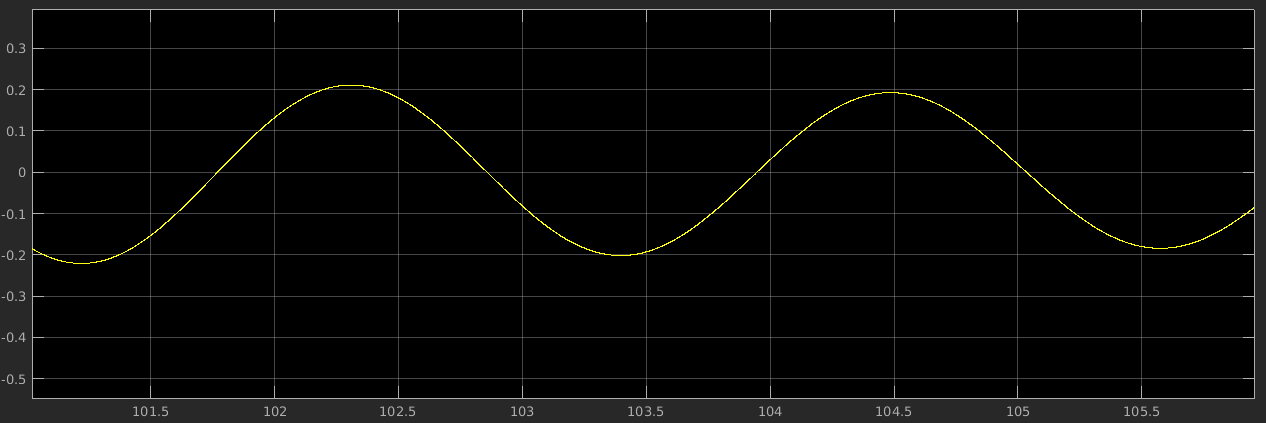
\includegraphics[width=\textwidth]{p5-proof}

\subsection*{Part 2}

FIXME


\section*{Problem 5: Oscillator}

FIXME


\section*{Problem 6: Geiger-Müller Counter}

FIXME


\end{document}
